\usepackage{tikz}
\usetikzlibrary{arrows.meta}

\tikzset{>={Latex[scale=1]}}

\newsavebox{\systemfig}

\savebox{\systemfig} {

	\begin{tikzpicture}[scale=.8, transform shape]
		\tikzstyle{every path} = [line width=1pt];
		
		\node (img) at (-.75, 0) {$\bxt$};
		\node[rectangle, draw, align=center] (spatial) at (1., 0) {Spatial\\ Attention};
		\node (glimpse) at (2.75, 0) {$\bgt$};
		
		\node[rectangle, draw] (v1) at (4, 0) {V1};
		
		\node[rectangle, draw, align=center] (dorsal) at (5.5, 1) {Dorsal\\ Stream};
		\node[rectangle, draw, align=center] (ventral) at (5.5, -1) {Ventral\\ Stream};
		
		\node (soft) at (7, 1) {$\bst$};
		\node (fmap) at (7,- 1) {$\bmapt$};
		\node (odot) at (7, 0) {$\odot$};
		\node (feat) at (8, 0) {$\bvt$};
		
		\node (hiddenm1) at (9.5, 1.25) {$\B{h}_{t-1}$};
		\node[rectangle, draw] (rnn) at (9.5, 0) {LSTM};
		\node (hidden) at (9.5, -1.25) {$\B{h}_t$};
		\node (ho) at (11, 0) {$\bot$};
		
		\node(concat) at (12.5, 0) {$\
			\begin{pmatrix}
			\tilde{\bs}_t \\ \bot
			\end{pmatrix}
			$};
		
		\node[rectangle, draw] (mlp) at (14, 0) {MLP};
		
		\node (app) at (14, 1) {$\bapp_{t+1}$};
		\node (bdelta) at (15.5, 0) {$\Delta \widehat{\bb}_t$};
		\node (att) at (14, -1) {$\ba_{t+1}$};
		
		\draw[->] (img) -- (spatial);
		\draw (spatial) -- (glimpse);
		\draw[->] (glimpse) -- (v1);
		\draw[->] (v1) to [out=90, in=180] (dorsal);
		\draw[->] (v1) to [out=-90, in=180] (ventral);
		
		
		\draw (ventral) to (fmap);
		\draw (dorsal) to (soft);
		\draw[->] (fmap) to (odot);
		\draw[->] (soft) to (odot);
		\draw (odot) to (feat);
		
		\draw[->, dash dot] (hiddenm1) to (rnn);
		\draw[->] (feat) to (rnn);
		\draw[->, dash dot] (rnn) to (hidden);
		\draw (rnn) to (ho);
		
		\draw[->] (ho) to (concat);
		\draw[->] (soft) to [out=25, in=135] (concat);
		\draw[->] (concat) to (mlp);
		
		\draw[->] (mlp) to (bdelta);
		\draw[->] (mlp) to (att);
		\draw[->] (mlp) to (app);
		
		\draw[->, dash dot] (app) to [out=165, in=20] (dorsal);
		\draw[->, dash dot] (att) to [out=-175, in=-35] (spatial);
	\end{tikzpicture}
}


\newsavebox{\archfig}

\savebox{\archfig} {

	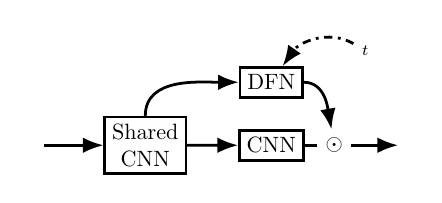
\begin{tikzpicture}[scale=.8, transform shape]
		\tikzstyle{every path} = [line width=1pt];
		
		\node (glimpse) at (1.75, 0) {$\bgt$};
		\node[rectangle, draw, align=center] (v1) at (3.5, 0) {Shared\\ CNN};
		
		
		\node[rectangle, draw, align=center] (dorsal) at (5.5, 1) {DFN};
		\node[rectangle, draw, align=center] (ventral) at (5.5, 0) {CNN};
		
		\node (odot) at (6.5, 0) {$\odot$};
		
		\node (feat) at (7.65, 0) {$\bvt$};
		\node (app) at (7., 1.5) {$\bapp_t$};
		
		
		\draw[->] (glimpse) to (v1);
		\draw[->] (v1) to [out=90, in=180] (dorsal);
		\draw[->] (v1) to [out=0, in=180] (ventral);
		\draw[->] (dorsal) to [out=0, in=100] (odot);
		\draw (ventral) to (odot);
		\draw[->] (odot) to (feat);
		
		\draw[->, dash dot] (app) to [out=150, in=55] (dorsal);
		

	\end{tikzpicture}
}